\chapter{Test Problem}
\label{chap:testprob}

Figure \ref{fig:testprob:flux} shows an example figure.

\begin{figure}[h!]
  \centering
  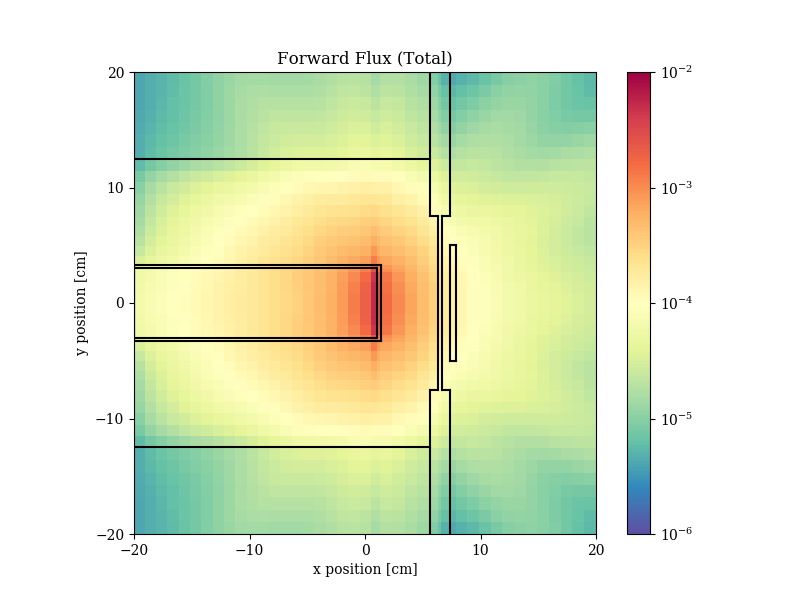
\includegraphics[width=1.0\textwidth]{content/scalar_flux_fwd_total.png}
  \caption[Short figure caption]{Long figure caption}
  \label{fig:testprob:flux}
\end{figure}

Table \ref{tab:testprob:mats} shows an example table.

\begin{table}[h]
  \centering
  \caption[Short table caption]{Long table caption}
  \label{tab:testprob:mats}
  \begin{tabular}{| c | c | c |}
    \hline
    \textbf{Material ID} & \textbf{Material} \\ \hline
     0 & Void                 \\ \hline
     1 & Air                  \\ \hline
     2 & Aluminum             \\ \hline
     3 & Beryllium            \\ \hline
     4 & Beryllium oxide      \\ \hline
     5 & Boron                \\ \hline
     6 & Graphite             \\ \hline
     7 & Copper               \\ \hline
     8 & Iron                 \\ \hline
     9 & Borated polyethylene \\ \hline
    10 & Polyethylene         \\ \hline
    11 & Heavy water          \\ \hline
    12 & Light water          \\ \hline
    13 & Uranium-235          \\ \hline
  \end{tabular}
\end{table}
